\documentclass{article}
\usepackage{amsmath, amssymb, graphicx}

\usepackage{graphicx} % 載入插圖套件
% 中文與字型設定
\usepackage{xeCJK}
\usepackage{fontspec}
\setCJKmainfont{Noto Serif CJK TC}  % ✅ Overleaf 支援
\xeCJKsetup{CJKecglue=\hspace{0.2em}}

% 段落縮排設定
\usepackage{indentfirst}
\setlength{\parindent}{2em}

% 頁面設定
\usepackage[a4paper, margin=2cm]{geometry}

% 超連結設定
\usepackage[hidelinks]{hyperref}
\usepackage{url}
\usepackage{array}
\usepackage{float}

\title{
  Lab1 Report\\[0.5em]
  \large Deep Learning\\
  \large Backpropagation
}

\author{
  姓名:陳科融 \\
  學號:314551010
}

\date{July 3, 2025}


\begin{document}

\maketitle
 
\section{Introduction}

    在本次實驗中,不使用 PyTorch 函式庫,而是僅基於 \texttt{NumPy} 函式庫,從零開始建構一個完整的神經網路。這個過程涵蓋了前向傳播(Forward Propagation)與反向傳播(Backpropagation)的完整設計與實作。其中,反向傳播演算法要求手動推導模型中每一層參數的偏微分公式,並將其轉化為具體的 Python 程式碼。

本專案設計的模型能夠成功對 \texttt{linear} 與 \texttt{XOR} 這兩種二維資料集進行有效的二元分類。為了提升實驗的效率與便利性,此專案額外開發了一個基於 \texttt{tkinter} 的圖形化使用者介面(GUI)。透過此介面,研究者可以快速調整訓練參數(如學習率、網路結構等),並一鍵啟動實驗,從而方便地進行多組參數的比較與結果分析。


\section{Implementation Details}

\subsection{Network Architecture}
本次實驗的核心為一個循序式(Sequential)神經網路模型,其架構允許開發者如堆疊積木般,依序加入不同的網路層。模型的基本建構單元是 \texttt{Linear} 層(即全連接層),它負責執行 \(y = Wx + b\) 的線性轉換,並與非線性的激勵函數交錯使用,賦予網路學習複雜模式的能力。

此網路設計的關鍵優勢在於其結構的靈活性。使用者可透過命令列參數 \texttt{--hidden-dims} 動態設定隱藏層的數量與各層的神經元數目。例如,輸入 \texttt{--hidden-dims 8 4} 將生成一個包含兩層隱藏層的網路,第一層有 8 個神經元,第二層則有 4 個。這種設計使得調整模型複雜度以適應不同任務需求變得相當便捷。

模型的輸入層維度固定為 2,用以處理 \texttt{linear} 與 \texttt{XOR} 資料集的二維特徵。輸出層則由單一神經元構成,並採用 \texttt{Sigmoid} 函數作為激勵,將輸出值壓縮至 (0, 1) 區間,使其能代表二元分類的機率。整個網路遵循標準的前向傳遞(Feedforward)流程,並透過反向傳播(Backpropagation)演算法進行訓練與權重更新。

\begin{figure}[htp]
    \centering
    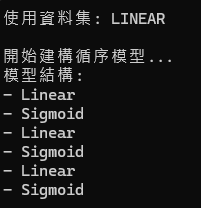
\includegraphics[width=5cm]{Lab01_report/img/2.1.png}
    \caption{模型架構圖}
    \label{fig:model}
\end{figure}

\subsection{Activation Functions}

\begin{itemize}
  \item \textbf{Sigmoid}: 此函數將輸出壓縮至 (0, 1) 之間,適合用於二元分類問題的輸出層。其數學形式為 \(\sigma(x) = \frac{1}{1 + e^{-x}}\),導數為 \(\sigma'(x) = \sigma(x)(1 - \sigma(x))\)。由於其輸出範圍有限,有助於穩定學習過程,但在深層網路中也可能出現梯度消失的問題。
\end{itemize}

\subsection{Backpropagation}
反向傳播是手動實作的,其核心邏輯如下:
\begin{enumerate}
  \item 從損失函數開始,計算對模型最終輸出的梯度 \(\partial L / \partial \hat{y}\)。
  \item 梯度會透過 \texttt{Sequential} 模型的 \texttt{backward} 方法,從最後一層反向傳播至第一層。
  \item 每一層實作了自己的 \texttt{backward} 方法。根據鏈式法則,該方法會接收來自後一層的梯度,計算該層內部參數(如權重 \(W\) 與偏置 \(b\))的梯度,並將計算出的梯度傳遞給前一層。
  \item 例如,在 \texttt{Linear} 層中,權重與偏置的梯度分別為 \(\partial L / \partial W = \mathbf{x}^T \cdot (\partial L / \partial y)\) 與 \(\partial L / \partial b = \sum (\partial L / \partial y)\)。
\end{enumerate}
最終,優化器(Optimizer)會使用這些計算出的梯度來更新模型的全部參數。

\begin{figure}[htp]
    \centering
    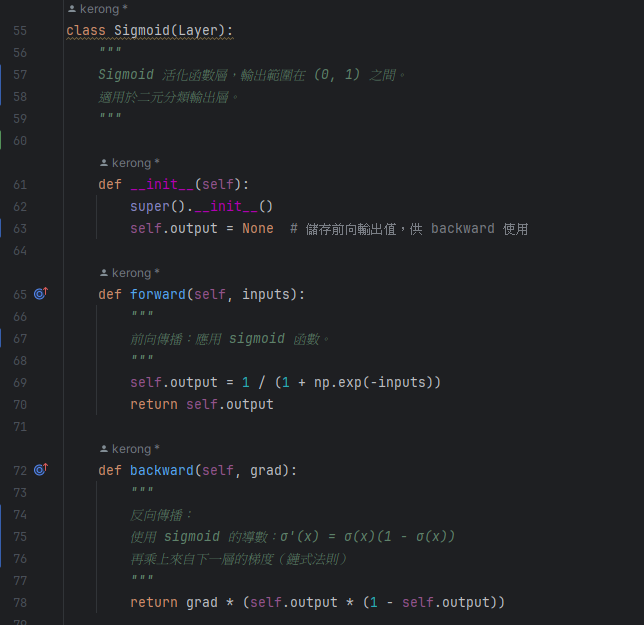
\includegraphics[width=12cm]{Lab01_report/img/2.2.png}
    \caption{激勵函數}
    \label{fig:activation}
\end{figure}

\subsection{Extra Implementation}
為了大幅提升模型的靈活性與實驗效率,本專案在滿足基本要求之外,進行了多項額外實作,實現了多種優化器、損失函數與一個完整的圖形化介面(GUI)。

所有可配置的選項皆整合為命令列參數,並透過 GUI 提供便捷的操作方式。下表詳細列出了所有支援的參數及其功能:

\begin{table}[h!]
\centering
\caption{模型支援的命令列參數}
\label{tab:params}
\begin{tabular}{|l|l|l|p{4.5cm}|}
\hline
\textbf{參數} & \textbf{預設值} & \textbf{選項} & \textbf{說明} \\
\hline
\texttt{--dataset} & \texttt{xor} & \texttt{linear}, \texttt{xor} & 選擇要使用的資料集。 \\
\hline
\texttt{--epochs} & \texttt{95000} & 任意正整數 & 設定訓練的週期總數。 \\
\hline
\texttt{--lr} & \texttt{0.1} & 任意正浮點數 & 設定學習率。 \\
\hline
\texttt{--hidden-dims} & \texttt{10 10} & 空白分隔的正整數 & 設定每個隱藏層的神經元數量。 \\
\hline
\texttt{--activation} & \texttt{sigmoid} & \texttt{sigmoid}, \texttt{relu}, \texttt{none} & 選擇隱藏層的激勵函數 (Bonus)。 \\
\hline
\texttt{--optimizer} & \texttt{sgd} & \texttt{sgd}, \texttt{gd}, \texttt{adam}, \texttt{adagrad} & 選擇優化器 (Bonus)。 \\
\hline
\texttt{--loss} & \texttt{bce} & \texttt{bce}, \texttt{mse}, \texttt{cross} & 選擇損失函數。 \\
\hline
\texttt{--momentum} & \texttt{0.0} & 0.0 到 1.0 & 設定 SGD 優化器的動量值。 \\
\hline
\texttt{--seed} & \texttt{1} & 任意正整數 & 設定隨機數種子,確保實驗可重複。 \\
\hline
\texttt{--log-interval} & \texttt{5000} & 任意正整數 & 每隔多少週期輸出一筆訓練日誌。 \\
\hline
\end{tabular}
\end{table}

此外,如圖 \ref{fig:gui} 所示的 GUI 介面,將所有參數選項視覺化,使用者無需記憶命令列指令,即可透過點選與輸入完成實驗配置,實現了一鍵啟動。

\begin{figure}[h!]
    \centering
    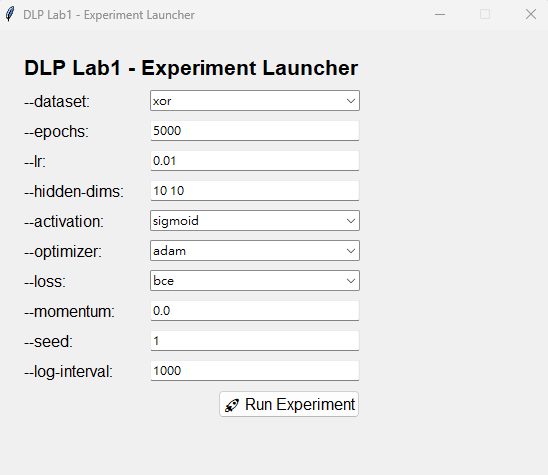
\includegraphics[width=8cm]{Lab01_report/img/2.4-1.png}
    \caption{基於 \texttt{tkinter} 的圖形化介面,整合了上表所有參數的設定功能。}
    \label{fig:gui}
\end{figure}



\clearpage  % 強制圖片浮動區結束,避免下一節卡進來

\section{Experimental Results}


\subsection{Screenshot and Comparison Figure}
此處將原始資料的分佈與模型的預測結果進行視覺化比較。如下圖所示,左側為真實的資料標籤(Ground Truth),右側為模型經過訓練後的預測結果(Prediction)。透過比較兩者,可以清晰地觀察到模型是否成功學習到了資料的分類邊界。

\begin{figure}[h]
    \centering
    \renewcommand{\arraystretch}{1.5}  % 增加行距讓表格看起來比較清楚
    \begin{tabular}{|>{\centering\arraybackslash}m{2cm}|c|}
        \hline
        \textbf{資料名稱} & \textbf{原始資料分佈與模型預測結果} \\
        \hline
        \large linear & 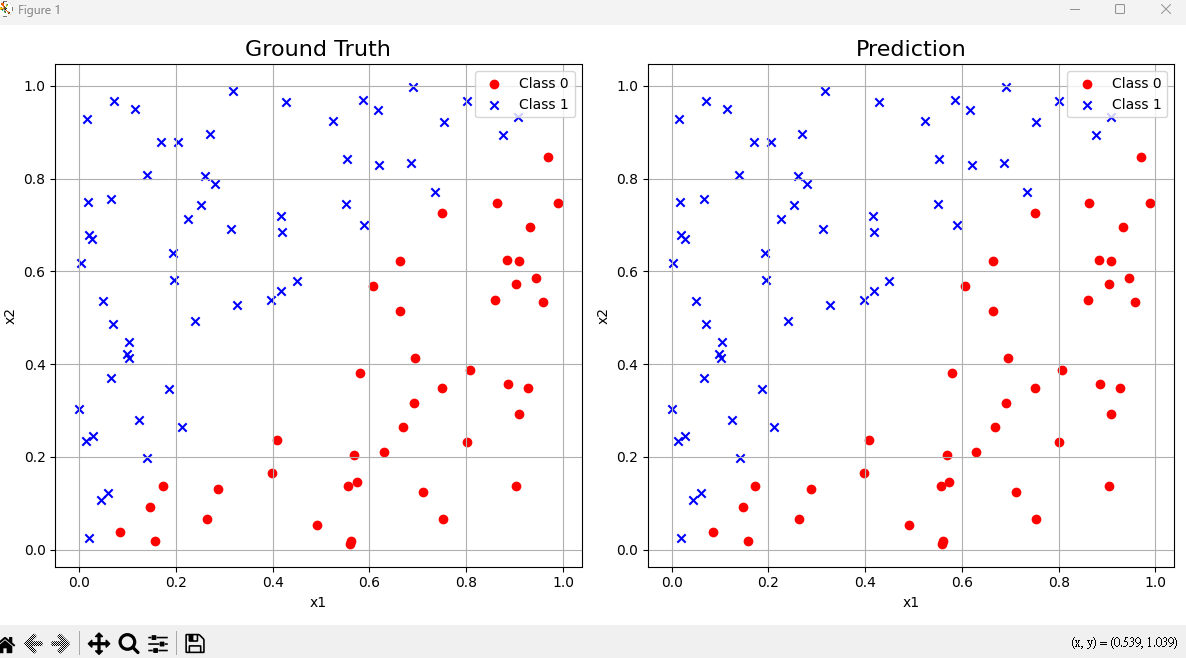
\includegraphics[width=8cm]{Lab01_report/img/3.1-linear.png} \\
        \hline
        \large xor & 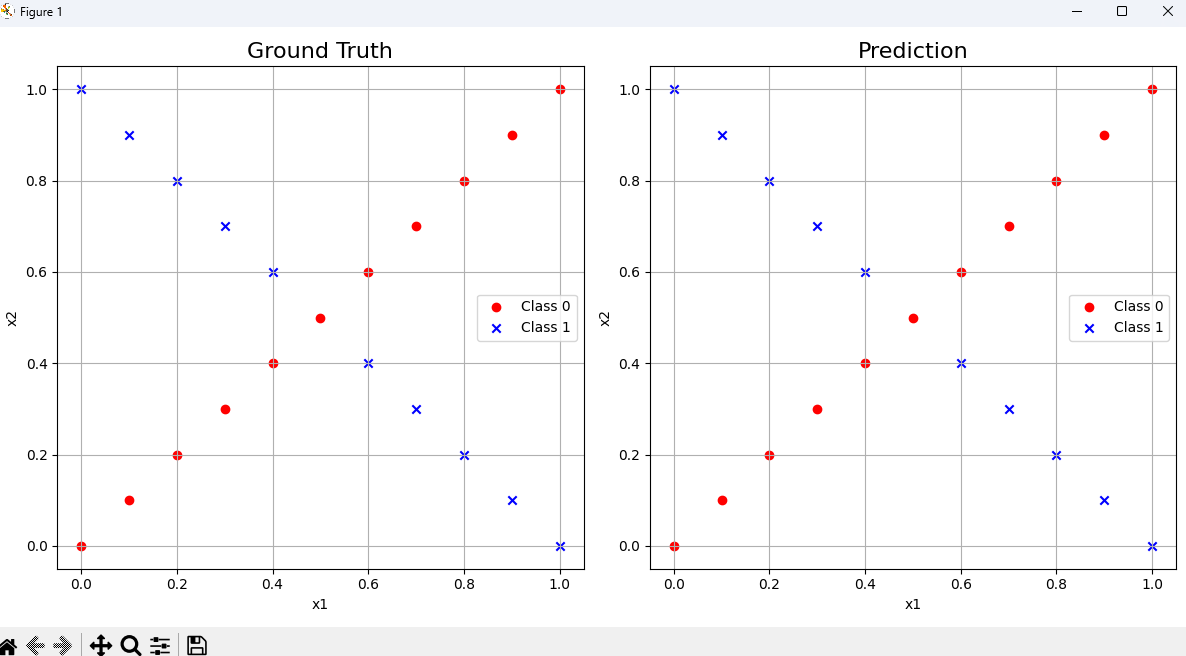
\includegraphics[width=8cm]{Lab01_report/img/3.1-xor.png} \\
        \hline
    \end{tabular}
    \caption{原始資料分佈與模型預測結果比較圖}
    \label{fig:comparison}
\end{figure}


\subsection{Prediction Accuracy}
模型在 \texttt{linear} 與 \texttt{XOR} 兩個資料集上均達到了 \textbf{100\%} 的預測準確率。此結果表明,網路架構與手動實作的反向傳播演算法能夠有效地學習並收斂。下表為兩個資料集的終端輸出,顯示了每一筆資料的預測詳情、最終的損失值(loss)與準確率(accuracy)。

\begin{table}[h!]
    \centering
    \caption{模型在測試資料上的預測準確率與損失值}
    \label{fig:accuracy}
    \begin{tabular}{|c|c|}
        \hline
        \textbf{Linear} & \textbf{XOR} \\
        \hline
        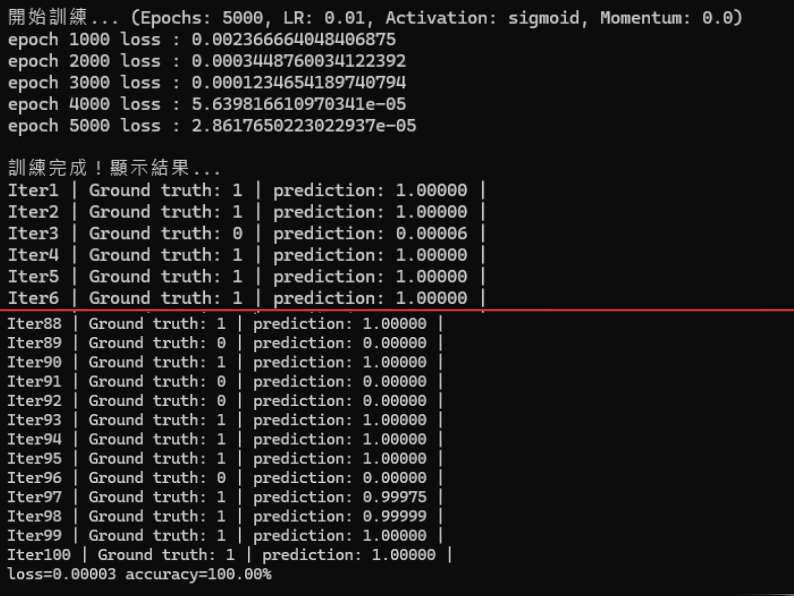
\includegraphics[width=0.45\textwidth]{Lab01_report/img/3.2-linear.png} & 
        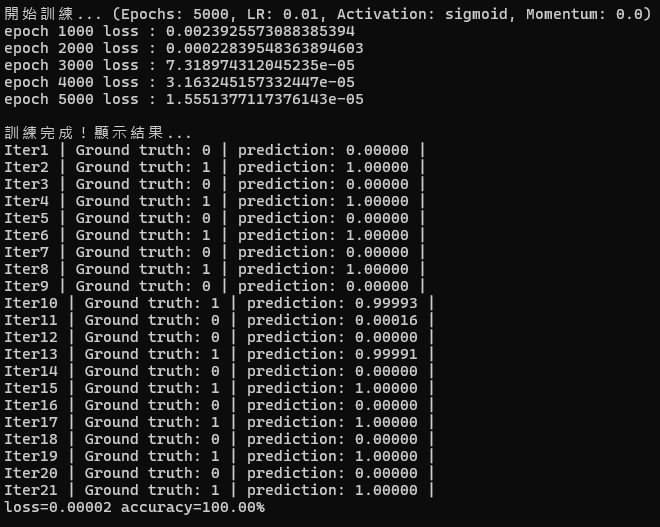
\includegraphics[width=0.45\textwidth]{Lab01_report/img/3.2-xor.png} \\
        \hline
    \end{tabular}
\end{table}

\subsection{Learning Curve}
學習曲線(Learning Curve)是評估模型訓練過程的重要指標。下圖展示了模型在訓練過程中,損失值(Loss)隨著訓練週期(Epoch)變化的情況。從圖中可以看出,損失值在訓練初期迅速下降,並在後期逐漸收斂至一個較低的值,顯示模型已穩定學習。

\begin{table}[h!]
    \centering
    \caption{訓練過程的損失函數變化圖(Loss-Epoch Curve)}
    \label{fig:loss_curve}
    \begin{tabular}{|c|c|}
        \hline
        \textbf{Linear} & \textbf{XOR} \\
        \hline
        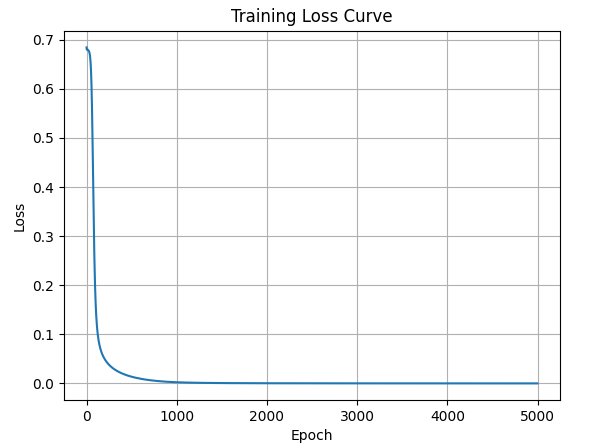
\includegraphics[width=0.45\textwidth]{Lab01_report/img/3.3-linear.png} &
        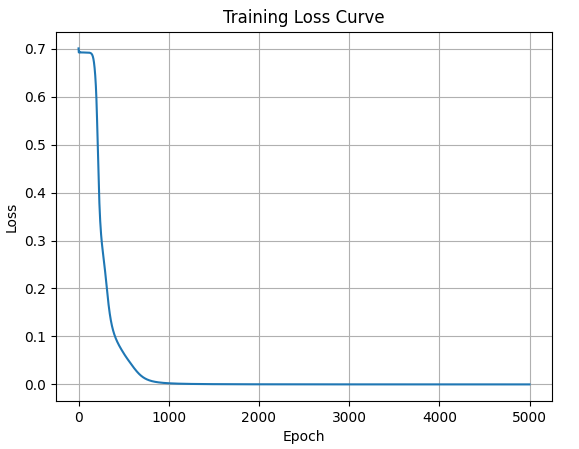
\includegraphics[width=0.45\textwidth]{Lab01_report/img/3.3-xor.png} \\
        \hline
    \end{tabular}
\end{table}

\subsection{Additional Results}
作為補充,此處詳細列出本次實驗所實作的 SGD with Momentum 以及三種損失函數及其梯度推導過程。

\subsubsection{SGD with Momentum}
除了標準的 SGD,本專案還實現了帶有動量(Momentum)的 SGD。動量旨在加速 SGD 在相關方向上的收斂並抑制振盪。下圖展示了使用 Momentum (0.9) 搭配 ReLU 激勵函數的實驗結果。

\begin{figure}[h!]
    \centering
    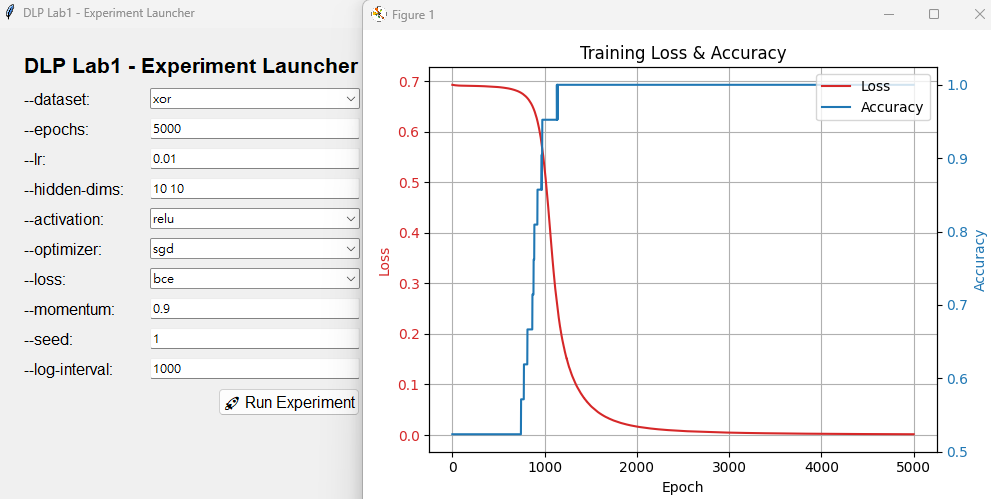
\includegraphics[width=1\textwidth]{Lab01_report/img/3.4.png}
    \caption{SGD with Momentum (0.9) and ReLU}
    \label{fig:momentum_result}
\end{figure}

\subsubsection{Mean Squared Error (MSE)}

MSE(均方誤差)是用來衡量模型預測值與真實值之間誤差的常見損失函數,常用於回歸(連續性)問題。其定義為:

\[
\text{MSE} = \frac{1}{n} \sum_{i=1}^{n} (\hat{y}_i - y_i)^2
\]

在反向傳播(Backpropagation)中,需要對每個預測值 \(\hat{y}_i\) 計算損失函數的偏微分。首先將 MSE 重寫為方便微分的形式:

\[
\frac{\partial}{\partial \hat{y}_i} \left( \frac{1}{n} \sum_{j=1}^n (\hat{y}_j - y_j)^2 \right)
= \frac{1}{n} \frac{\partial}{\partial \hat{y}_i} (\hat{y}_i - y_i)^2
\]

因為只有第 \(i\) 項與 \(\hat{y}_i\) 有關,其他項的偏微分為零。進一步計算:

\[
\frac{\partial}{\partial \hat{y}_i} (\hat{y}_i - y_i)^2 = 2(\hat{y}_i - y_i)
\]

因此,對每個預測值的梯度為:

\[
\frac{\partial \text{MSE}}{\partial \hat{y}_i}
= \frac{2}{n} (\hat{y}_i - y_i)
\]

梯度公式:

\[
\boxed{
\nabla_{\hat{\mathbf{y}}} \text{MSE}
= \frac{2}{n} (\hat{\mathbf{y}} - \mathbf{y})
}
\]


\subsubsection{Cross Entropy Loss}

交叉熵(Cross Entropy)常用於多類別分類問題,用以衡量模型預測的機率分布與真實標籤分布之間的差異,假設模型輸出 logits 為 \(\mathbf{z} = (z_1, z_2, \ldots, z_C)\),
經 softmax 轉換成預測機率:

\[
\hat{y}_k = \frac{e^{z_k}}{\sum_{j=1}^C e^{z_j}}
\]

交叉熵損失函數為:

\[
L = - \sum_{c=1}^C y_c \log(\hat{y}_c)
\]

其中 \(y_c\) 為真實標籤。

對 logits \(z_k\) 求導數,利用鏈式法則:

\[
\frac{\partial L}{\partial z_k} 
= \sum_{j=1}^C \frac{\partial L}{\partial \hat{y}_j} \cdot \frac{\partial \hat{y}_j}{\partial z_k}
\]

其中,

\[
\frac{\partial L}{\partial \hat{y}_j} = - \frac{y_j}{\hat{y}_j}
\]

且 softmax 的偏微分為:

\[
\frac{\partial \hat{y}_j}{\partial z_k} = \hat{y}_j (\delta_{jk} - \hat{y}_k)
\]

\(\delta_{jk}\) 為克羅內克 delta,當 \(j=k\) 時為1,否則為0。

代入整理得:

\[
\begin{aligned}
\frac{\partial L}{\partial z_k}
&= \sum_{j=1}^C \left(- \frac{y_j}{\hat{y}_j}\right) \hat{y}_j (\delta_{jk} - \hat{y}_k) \\
&= \sum_{j=1}^C - y_j (\delta_{jk} - \hat{y}_k) \\
&= - y_k (1 - \hat{y}_k) - \sum_{j \neq k} y_j (- \hat{y}_k) \\
&= - y_k + y_k \hat{y}_k + \hat{y}_k \sum_{j \neq k} y_j \\
&= - y_k + \hat{y}_k \sum_{j=1}^C y_j \\
&= - y_k + \hat{y}_k \cdot 1 \quad (\because \sum_{j=1}^C y_j = 1) \\
&= \hat{y}_k - y_k
\end{aligned}
\]


此推導結果是深度學習中 softmax 與交叉熵損失結合後梯度公式:

\[
\boxed{
\frac{\partial L}{\partial z_k} = \hat{y}_k - y_k
}
\]


\subsubsection{Binary Cross Entropy Loss}

Binary Cross Entropy(BCE,二元交叉熵)損失函數用於衡量二分類模型預測機率與實際標籤之間的差異,其定義如下:

\[
L = - \frac{1}{n} \sum_{i=1}^n \left[ y_i \log(\hat{y}_i) + (1 - y_i) \log(1 - \hat{y}_i) \right]
\]

其中:
\begin{itemize}
  \item \(n\):樣本數
  \item \(y_i \in \{0,1\}\):第 \(i\) 筆樣本的真實標籤
  \item \(\hat{y}_i \in (0,1)\):模型對第 \(i\) 筆樣本預測為正類的機率(通常為 sigmoid 輸出)
\end{itemize}

在反向傳播時,需對每一筆預測值 \(\hat{y}_i\) 計算偏微分。推導如下:

\[
\begin{aligned}
\frac{\partial L}{\partial \hat{y}_i}
&= - \frac{1}{n} \cdot \frac{\partial}{\partial \hat{y}_i} \left[ y_i \log(\hat{y}_i) + (1 - y_i) \log(1 - \hat{y}_i) \right] \\
&= - \frac{1}{n} \left( \frac{y_i}{\hat{y}_i} - \frac{1 - y_i}{1 - \hat{y}_i} \right)
\end{aligned}
\]

因此,二元交叉熵的梯度公式為:

\[
\boxed{
\frac{\partial L}{\partial \hat{y}_i}
= - \frac{1}{n} \left( \frac{y_i}{\hat{y}_i} - \frac{1 - y_i}{1 - \hat{y}_i} \right)
}
\]

\section{Discussions}

\subsection{Learning Rates}
本節比較不同學習率(Learning Rate)對模型收斂速度與最終表現的影響。當學習率過高時,模型在訓練初期損失值會劇烈震盪,甚至無法收斂;反之,當學習率過低時,雖然模型能穩定下降,但收斂速度極慢,需要耗費大量訓練時間。實驗證明,選擇一個適中的學習率至關重要,它能在保證收斂穩定性的前提下,最快地找到損失函數的最小值。下表展示了不同學習率設定下的學習曲線:

\begin{table}[h!]
    \centering
    \caption{不同學習率下的學習曲線比較}
    \label{tab:lr_comparison}
    \begin{tabular}{|c|c|}
        \hline
        \textbf{Linear Dataset} & \textbf{XOR Dataset} \\
        \hline
        \begin{tabular}{@{}c@{}}
            \textbf{LR = 0.1} \\
            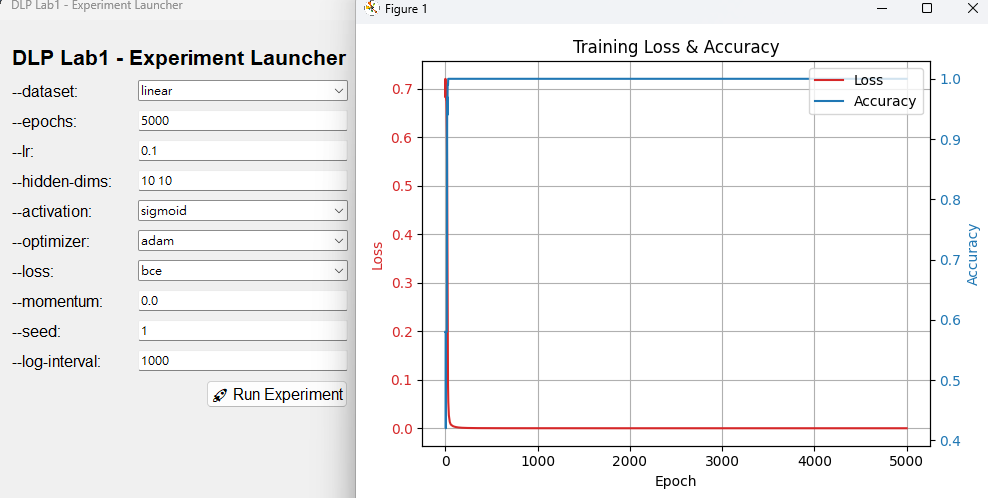
\includegraphics[width=0.4\textwidth]{Lab01_report/img/4.1linear_0.1.png} \\
            \textbf{LR = 0.01} \\
            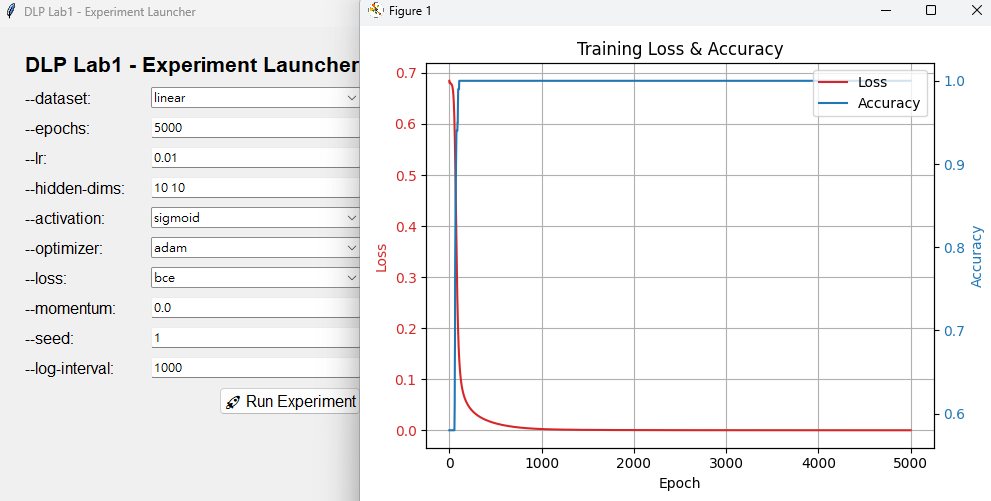
\includegraphics[width=0.4\textwidth]{Lab01_report/img/4.1linear_0.01.png} \\
            \textbf{LR = 0.001} \\
            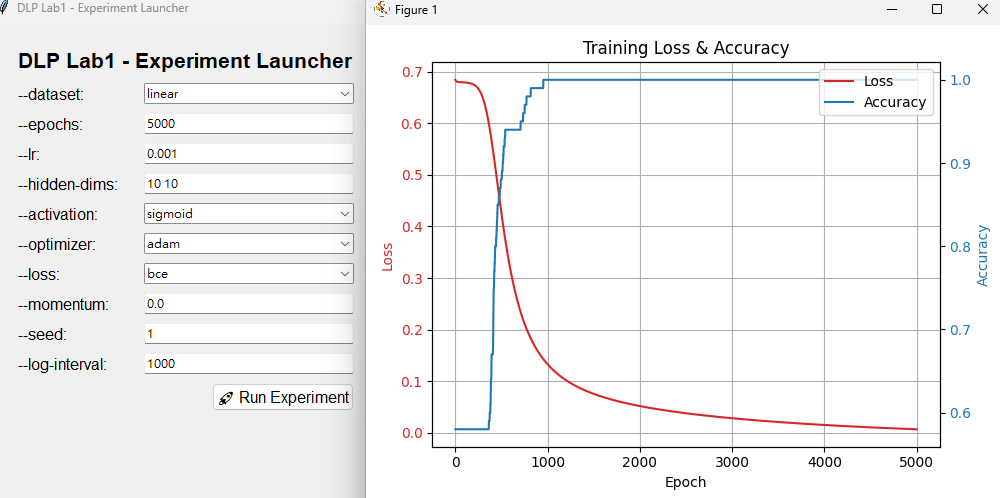
\includegraphics[width=0.4\textwidth]{Lab01_report/img/4.1linear_0.001.png}
        \end{tabular}
        &
        \begin{tabular}{@{}c@{}}
            \textbf{LR = 0.1} \\
            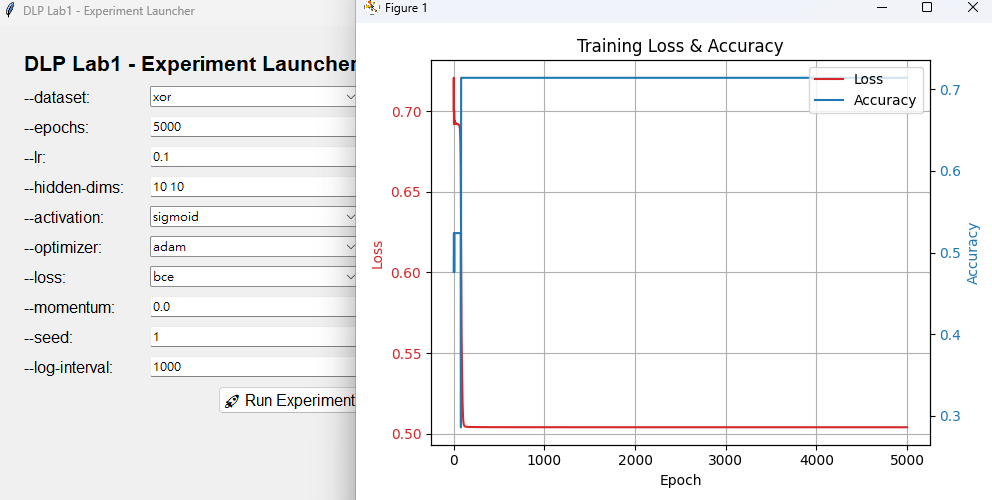
\includegraphics[width=0.4\textwidth]{Lab01_report/img/4.1xor_0.1.png} \\
            \textbf{LR = 0.01} \\
            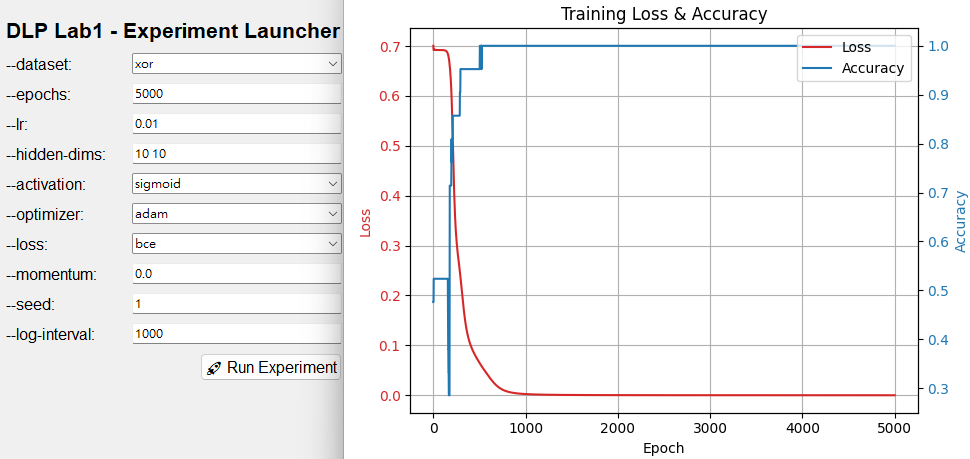
\includegraphics[width=0.4\textwidth]{Lab01_report/img/4.1xor_0.01.png} \\
            \textbf{LR = 0.001} \\
            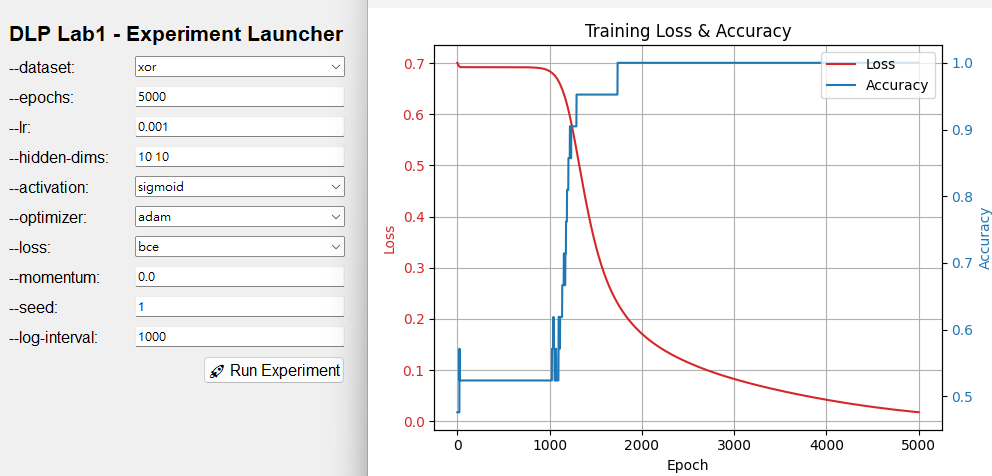
\includegraphics[width=0.4\textwidth]{Lab01_report/img/4.1xor_0.001.png}
        \end{tabular} \\
        \hline
    \end{tabular}
\end{table}

\subsection{Number of Hidden Units}
隱藏層神經元的數量直接影響模型的表達能力。在 XOR 問題上,若神經元數量過少(例如每層僅 2 個),模型可能難以學習到非線性的決策邊界,導致準確率下降。而增加神經元數量(例如每層 10 個或更多)能賦予模型更強的擬合能力,使其輕鬆解決 XOR 問題。然而,過多的神經元也可能增加過擬合的風險與不必要的計算成本,因此需要根據問題的複雜度進行權衡。下表展示了不同隱藏層大小設定下的決策邊界:

\begin{table}[h!]
    \centering
    \caption{不同隱藏層單元數下的決策邊界}
    \label{tab:hidden_units_comparison}
    \begin{tabular}{|c|c|c|}
        \hline
        \textbf{4-8 Units} & \textbf{50-50 Units} & \textbf{100-100 Units} \\
        \hline
        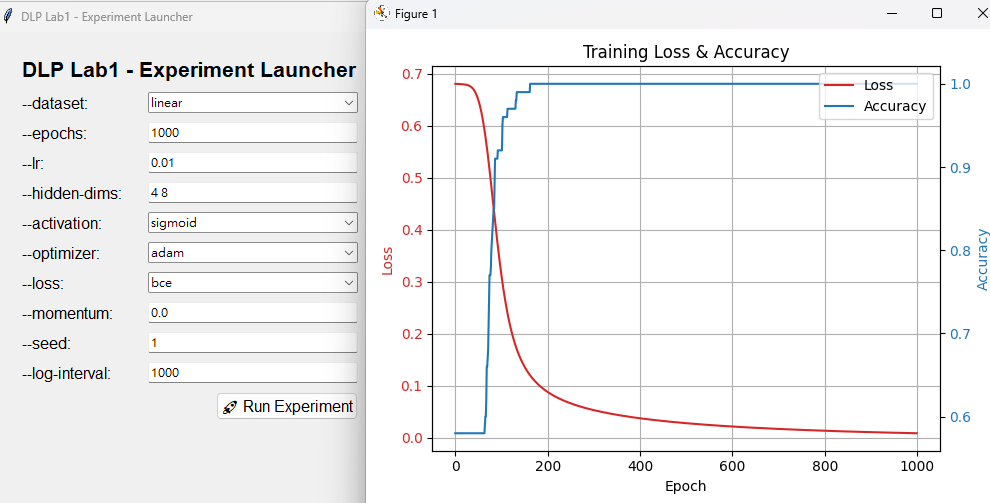
\includegraphics[width=0.3\textwidth]{Lab01_report/img/4.2_4-8.png} &
        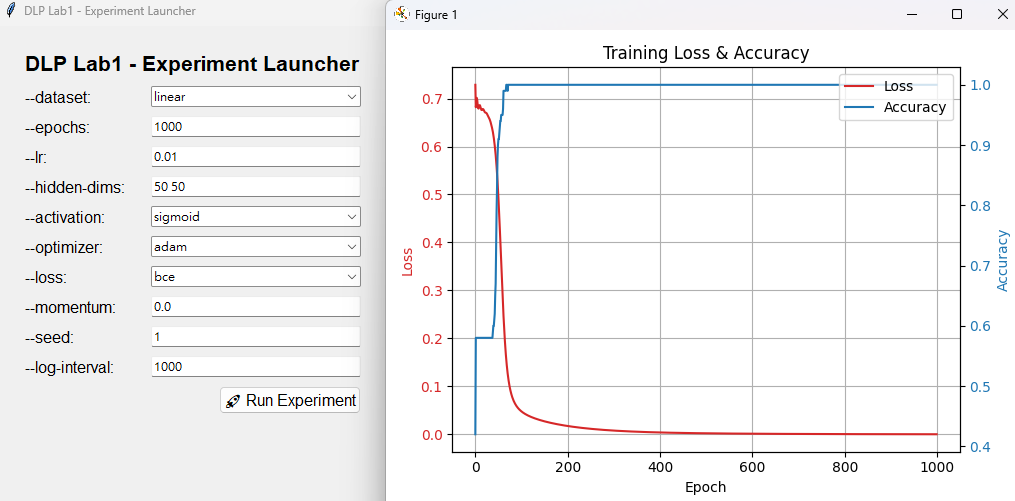
\includegraphics[width=0.3\textwidth]{Lab01_report/img/4.2_50-50.png} &
        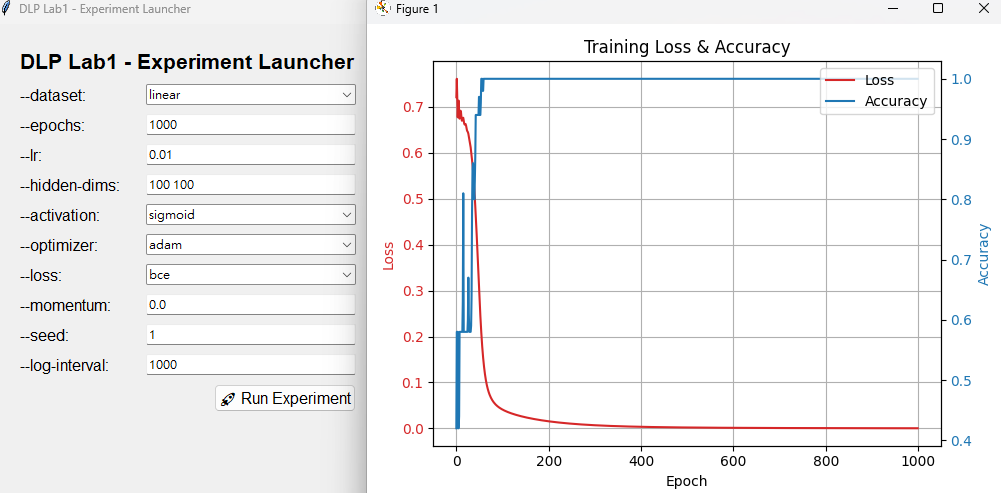
\includegraphics[width=0.3\textwidth]{Lab01_report/img/4.2_100-100.png} \\
        \hline
    \end{tabular}
\end{table}

\subsection{Without Activation Functions}
為了驗證非線性激勵函數的必要性,此處進行了一組移除所有隱藏層激勵函數的對照實驗。在這種設定下,整個神經網路,無論有多少層,都會退化為一個單純的線性模型,因為多個線性轉換的堆疊本質上仍然是線性的。

實驗結果正如預期:
\begin{itemize}
    \item 對於 \texttt{linear} 資料集,由於其本身就是線性可分的,模型依然能達到 100\% 的準確率。
    \item 然而,在 \texttt{XOR} 資料集上,模型完全無法學習其非線性模式。如下圖所示,模型的準確率在 50\% 左右停滯不前,損失值也無法有效下降,這與隨機猜測的結果無異。
\end{itemize}
這項實驗有力地證明了激勵函數在賦予神經網路學習複雜、非線性關係能力中的不可或缺性。沒有它,網路就無法解決像 XOR 這樣的基本非線性問題。

\begin{figure}[h!]
    \centering
    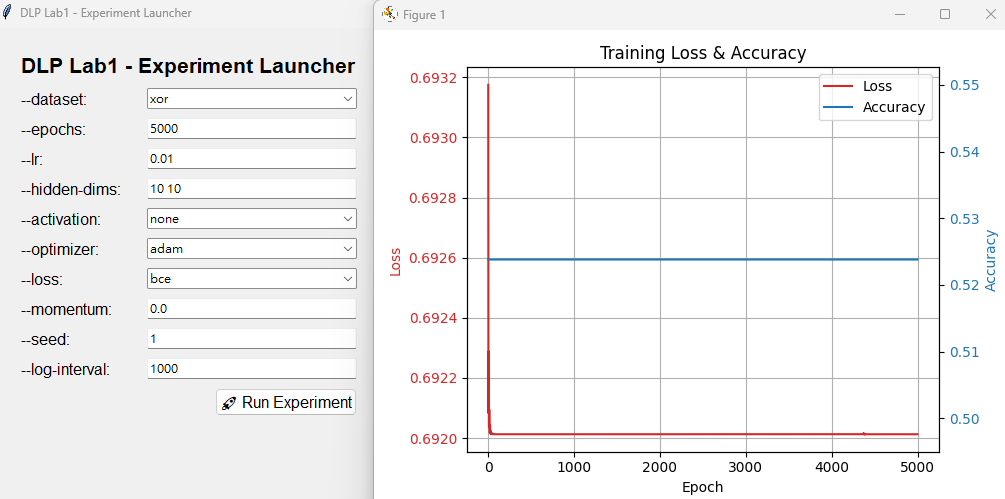
\includegraphics[width=0.8\textwidth]{Lab01_report/img/4.3.png}
    \caption{在 XOR 資料集上移除激勵函數的訓練結果}
    \label{fig:no_activation}
\end{figure}

\subsection{Extra Implementation Discussions}
本次專案中的額外實作,極大地提升了實驗的深度與廣度。所建立的模組化框架,允許自由組合不同的激勵函數、優化器與損失函數,進行更深入的比較分析。

例如,下表展示了兩種不同的組合:
\begin{itemize}
    \item \textbf{ReLU + SGD (Momentum=0.9) + Cross Entropy Loss}: 這個組合在訓練過程中表現出較快的收斂速度,動量的加入有助於模型跳出局部最小值。
    \item \textbf{ReLU + Adagrad + MSE Loss}: Adagrad 作為一種自適應學習率算法,能夠在訓練過程中自動調整學習率,使其在處理不同特徵時更具彈性。
\end{itemize}


\begin{table}[h!]
    \centering
    \caption{不同優化器、激勵函數與損失函數組合的實驗結果}
    \label{tab:extra_impl_comparison}
    \begin{tabular}{|c|c|}
        \hline
        \textbf{ReLU + SGD (Momentum=0.9) + Cross Entropy} & \textbf{ReLU + Adagrad + MSE} \\
        \hline
        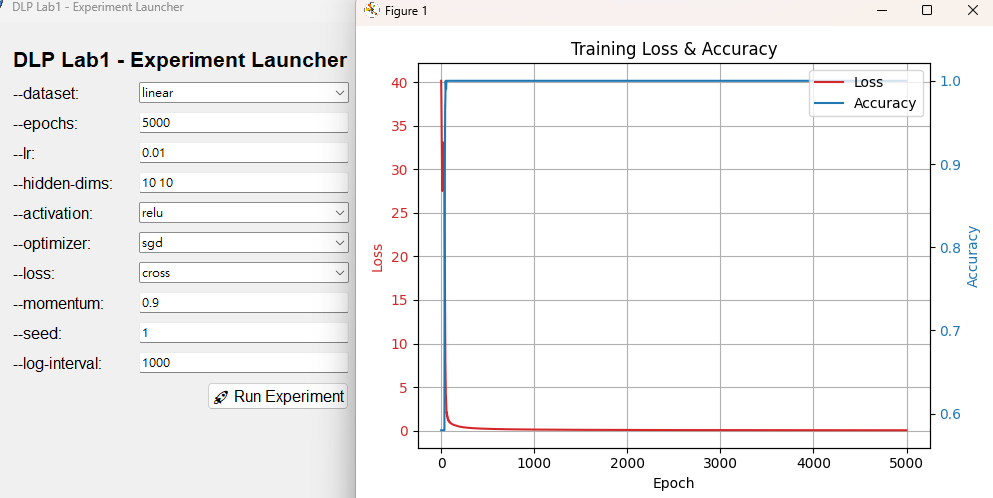
\includegraphics[width=0.45\textwidth]{Lab01_report/img/4.4_relu_sgd_cross.png} &
        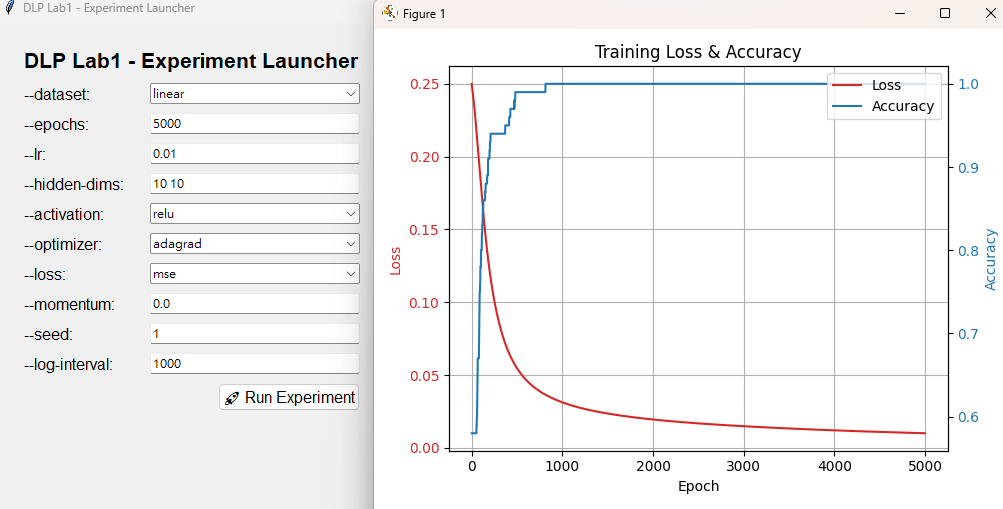
\includegraphics[width=0.45\textwidth]{Lab01_report/img/4.4_relu_adagrad_mse.png} \\
        \hline
    \end{tabular}
\end{table}

\section{Questions}

\subsection{Purpose of Activation Functions}
激勵函數(Activation Function)在神經網路中扮演著至關重要的角色,其主要目的有以下幾點:
\begin{itemize}
    \item \textbf{引入非線性:} 這是激勵函數最核心的功能。如果沒有激勵函數,多層神經網路本質上只是一個線性模型,無論網路有多深,都只能學習線性關係。例如,在本次實驗的 XOR 問題中,若移除激勵函數,模型將無法找到非線性的決策邊界。激勵函數的引入,使得網路能夠擬合複雜的非線性模式。
    \item \textbf{控制輸出範圍:} 某些激勵函數能將神經元的輸出限制在特定範圍內。例如,Sigmoid 函數會將輸出壓縮到 (0, 1) 之間,使其能被解釋為機率,這在二元分類或機率預測任務中非常有用。
    \item \textbf{影響梯度傳播:} 激勵函數的導數直接影響反向傳播中梯度的計算。選擇不同的激勵函數(如 ReLU)可以緩解梯度消失(Vanishing Gradients)問題,從而讓更深層的網路也能被有效訓練。
\end{itemize}

\subsection{Effect of Learning Rate}
學習率(Learning Rate)是控制模型權重更新幅度的超參數,其設定對訓練過程有著決定性的影響:
\begin{itemize}
    \item \textbf{學習率過大:} 如果學習率設置得太大,權重更新的步長就會過長。在梯度下降過程中,這很可能導致更新步伐「跨過」損失函數的谷底,造成損失值在最小值附近劇烈震盪,甚至可能導致損失值不減反增,模型完全無法收斂。
    \item \textbf{學習率過小:} 如果學習率設置得太小,權重更新的步長就會非常微小。這會導致模型收斂速度極其緩慢,需要耗費大量的訓練時間與計算資源。此外,過小的學習率也可能讓模型陷入局部最小值(Local Minima)或鞍點(Saddle Point),難以找到全局最優解。
\end{itemize}


\subsection{Purpose of Weights and Biases}
權重(Weights)與偏置(Biases)是神經網路中的核心可學習參數,它們共同決定了模型的功能:
\begin{itemize}
    \item \textbf{權重 (Weights):} 權重定義了神經元之間連接的強度。在一個神經元中,每個輸入特徵都對應一個權重,這個權重衡量了該特徵對於最終輸出的重要性。在訓練過程中,神經網路透過反向傳播演算法,不斷調整權重的值,其本質就是學習如何從輸入數據中提取有用的模式。可以說,權重儲存了模型從資料中學到的「知識」。
    \item \textbf{偏置 (Biases):} 偏置為每個神經元提供了一個可學習的常數項,它與輸入值無關。其主要作用是調整激勵函數的觸發閾值。如果沒有偏置,激勵函數的中心點將永遠固定在原點。偏置的存在,賦予了模型更大的靈活性,允許它將決策邊界向左或向右平移,從而更好地擬合數據。
\end{itemize}
總結來說,權重負責調整輸入信號的「斜率」,而偏置則負責調整「截距」,兩者共同決定了神經元的輸出。

\section{Bonus}

\subsection{Optimizers}
優化器就是不同的梯度下降方法,會根據學習率(Learning Rate)的大小來決定模型在
訓練時的時間與速度。若 Learning Rate 太小,會花費過多時間在學習,反之,則容  
易造成 Overfitting。

\subsubsection{Gradient Descent(GD)}
梯度其實就是函數的斜率,代表函數在某點的變化率。 在單變數迴歸中,權重即為斜率;而在多變數迴歸或神經網路中,則需對每個參數分別求偏微分,得到對應的梯度值。
\begin{figure}[H]
    \centering
    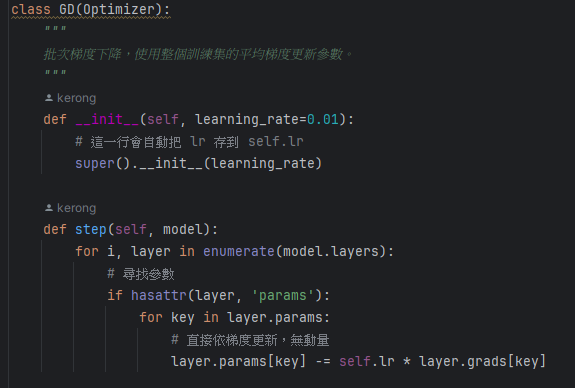
\includegraphics[width=0.6\textwidth]{Lab01_report/img/6.1GD.png}
    \caption{GD Implementation}
    \label{fig:gd_code}
\end{figure}


\subsubsection{Stochastic Gradient Descent with Momentum(SGD)}

隨機梯度下降(Stochastic Gradient Descent, SGD)是一種常見的優化方法,其目標是最小化損失函數 \(J(\theta)\)。基本的 SGD 僅依賴當前梯度來更新參數,但若加入「動量(Momentum)」機制,則能提升收斂速度並減少震盪。

\textbf{動量的核心概念是:保留過去梯度的指向,透過「速度」引導參數向更穩定的方向更新。}

其更新公式為:

\[
\begin{aligned}
v_t &= \mu v_{t-1} - \eta \nabla_\theta J(\theta) \\
\theta &= \theta + v_t
\end{aligned}
\]

\begin{description}
  \item[\(\theta\)] 模型的參數向量。
  \item[\(\eta\)] 學習率(learning rate)。
  \item[\(\mu\)] 動量係數(momentum coefficient)。
  \item[\(v_t\)] 當前的速度(velocity)。
  \item[\(\nabla_\theta J(\theta)\)] 損失函數對參數的梯度。
\end{description}

第一式會根據當前梯度與過去速度計算新的速度,第二式則將此速度應用於參數更新。

使用動量的 SGD 方法,能有效降低梯度震盪,尤其在深度網路或不平坦的損失曲面上,能加快收斂並提升訓練穩定性。
\begin{figure}[H]
    \centering
    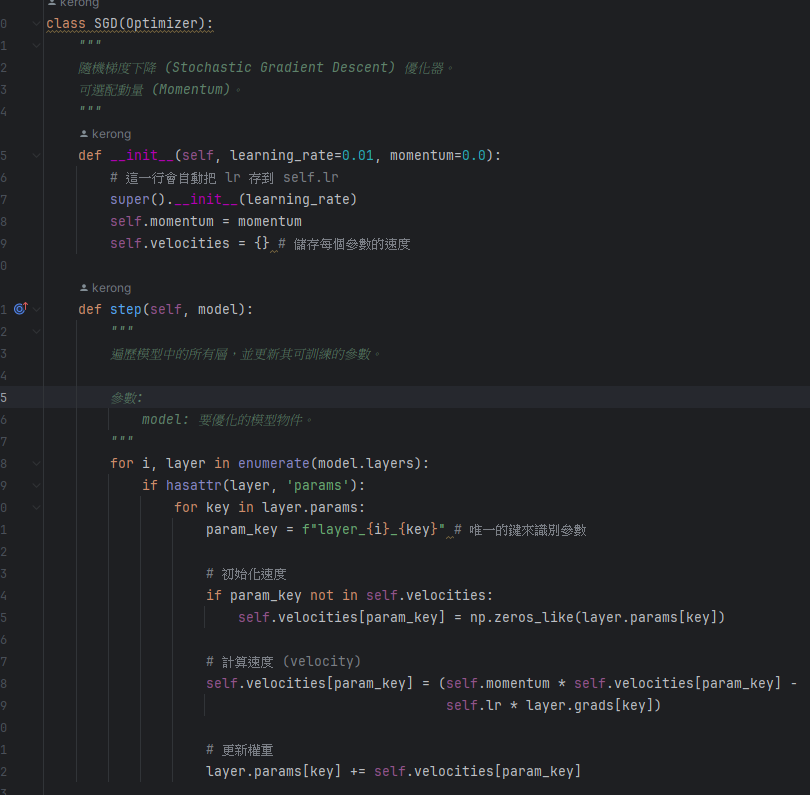
\includegraphics[width=0.8\textwidth]{Lab01_report/img/6.1SGD.png}
    \caption{SGD with Momentum Implementation}
    \label{fig:sgd_code}
\end{figure}


\subsubsection{Adaptive Moment Estimation(Adam)}

Adam是一種結合 Momentum(動量)與 RMSProp(均方根自適應學習率)的優化方法,能根據歷史梯度自動調整每個參數的學習率,並透過偏差修正讓初期估計更準確,進而提升訓練穩定性與收斂速度。

Adam 的更新步驟如下:

\begin{itemize}
  \item 初始化:一階矩估計 \(m_0 = 0\)、二階矩估計 \(v_0 = 0\)、時間步長 \(t = 0\)
  \item 超參數設定:\(\beta_1 = 0.9\)、\(\beta_2 = 0.999\)、\(\epsilon = 10^{-8}\)
\end{itemize}

每一步的參數更新公式如下:

\[
\begin{aligned}
t &\leftarrow t + 1 \\
g_t &= \nabla_\theta J(\theta_t) \\
m_t &= \beta_1 \cdot m_{t-1} + (1 - \beta_1) \cdot g_t \\
v_t &= \beta_2 \cdot v_{t-1} + (1 - \beta_2) \cdot g_t^2 \\
\hat{m}_t &= \frac{m_t}{1 - \beta_1^t} \\
\hat{v}_t &= \frac{v_t}{1 - \beta_2^t} \\
\theta_{t+1} &= \theta_t - \eta \cdot \frac{\hat{m}_t}{\sqrt{\hat{v}_t} + \epsilon}
\end{aligned}
\]


\begin{figure}[H]
    \centering
    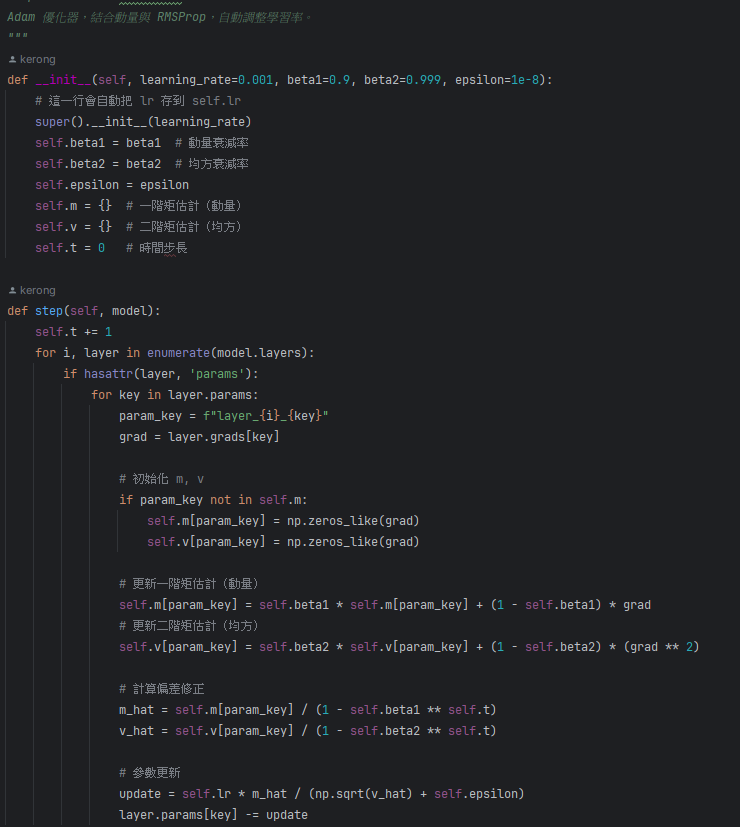
\includegraphics[width=0.6\textwidth]{Lab01_report/img/6.1adam.png}
    \caption{Adam Implementation}
    \label{fig:adam_code}
\end{figure}

\subsubsection{Adaptive Gradient Algorithm(Adagrad)}

Adagrad是一種自適應學習率的優化方法。與 SGD 及 Momentum 使用固定學習率不同,Adagrad 會根據每個參數的歷史梯度,自動調整其對應的學習率。該演算法能在訓練過程中約束學習率,依據每個參數的梯度大小進行調整。

\textbf{核心思想:}
當梯度在前期較小(例如平坦區域)時,學習率會被放大,加快訓練收斂速度;而當梯度較大(例如陡峭區域)時,學習率會被縮小,避免振盪。

其更新公式如下:

\[
\begin{aligned}
g_t &= \nabla_\theta J(\theta_t) \\
r_t &= r_{t-1} + g_t^2 \\
\theta_{t+1} &= \theta_t - \frac{\eta}{\sqrt{r_t} + \epsilon} \cdot g_t
\end{aligned}
\]

\begin{description}
  \item[\(\theta\)] 表示模型參數向量。
  \item[\(g_t\)] 是當前梯度 \(\nabla_\theta J(\theta_t)\)。
  \item[\(r_t\)] 是歷史平方梯度的累積值。
  \item[\(\eta\)] 是初始學習率(learning rate)。
  \item[\(\epsilon\)] 是防止除以零的小常數(通常為 \(10^{-8}\))。
\end{description}
\begin{figure}[H]
    \centering
    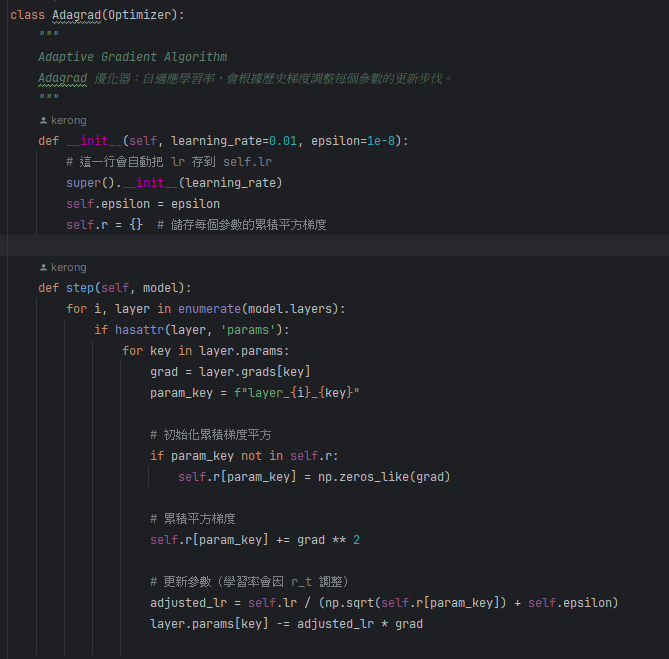
\includegraphics[width=0.8\textwidth]{Lab01_report/img/6.1adagrad.png}
    \caption{Adagrad Implementation}
    \label{fig:adagrad_code}
\end{figure}

\subsection{Activation Functions}
除了 Sigmoid 之外,本專案也實作了 ReLU 作為另一種激勵函數選項。

\subsubsection{Rectified Linear Unit (ReLU)}
ReLU (Rectified Linear Unit) 是目前深度學習中最受歡迎的激勵函數之一,因其簡單、高效且能有效緩解梯度消失問題。

\textbf{數學定義:}
其數學形式非常簡潔:
\[
\text{ReLU}(x) = \max(0, x)
\]
這意味著,當輸入 \(x\) 為正數時,輸出就是 \(x\) 本身;當輸入為負數時,輸出為 0。

\textbf{梯度推導:}
ReLU 的導數同樣非常簡單,這使得其在反向傳播中的計算十分高效:
\[
\frac{d}{dx} \text{ReLU}(x) =
\begin{cases}
1 & \text{if } x > 0 \\
0 & \text{if } x \le 0
\end{cases}
\]
在實作中,當 \(x=0\) 時的梯度可以定義為 0 或 1,通常定義為 0。這種分段線性的特性避免了 Sigmoid 函數在飽和區(輸入值過大或過小)梯度趨近於零的問題,從而讓深層網路的訓練更加穩定。

\begin{figure}[H]
    \centering
    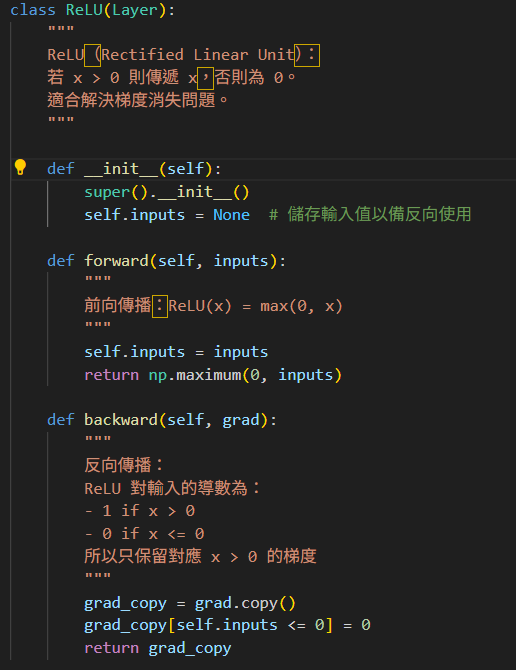
\includegraphics[width=0.6\textwidth]{Lab01_report/img/6.2_relu.png}
    \caption{ReLU Implementation}
    \label{fig:relu_code}
\end{figure}


\section{參考資料}
\begin{itemize}
  \item \href{https://github.com/hank891008/Deep-Learning}{https://github.com/hank891008/Deep-Learning}(學習如何將 function 分層結構化)
  \item \href{https://github.com/KJLdefeated/NYCU_DLP_2024}{https://github.com/KJLdefeated/NYCU\_DLP\_2024}(學習如何撰寫 Overleaf LaTeX 文件)
  \item \href{https://github.com/shflte/nycu-dlp-2024-summer}{https://github.com/shflte/nycu-dlp-2024-summer}(學習程式邏輯)
  \item \href{https://hackmd.io/@ivorchu/rJ3DPsgud}{https://hackmd.io/@ivorchu/rJ3DPsgud}(深度學習筆記)
  \item \href{https://youtube.com/playlist?list=PLJV_el3uVTsMhtt7_Y6sgTHGHp1Vb2P2J&si=17mjOUjyCP2tRXVk}{youtube機器學習教學影片-李弘毅教授}
  \item \href{https://blog.csdn.net/wzk4869/article/details/131409675}{https://blog.csdn.net/wzk4869/article}(損失函數相關參考資料)
  \item \href{https://blog.csdn.net/xpy870663266/article/details/104794371}{https://blog.csdn.net/xpy870663266/article}(優化器參考資料)
  \item \href{https://www.geeksforgeeks.org/machine-learning/activation-functions-neural-networks/}{https://www.geeksforgeeks.org/machine-learning/activation-functions-neural-networks/}(激勵函數相關參考資料)
  \item 使用 AI 工具輔助:
  \begin{itemize}
    \item ChatGPT GPT-4o(Free Plan)
    \item Google AI Gemini 2.5 Pro
    \item VS Code 搭配 Copilot(GPT-4o)
  \end{itemize}
\end{itemize}

\end{document}
